\documentclass[11pt]{IEEEtran}

\usepackage{cite}				% Used to cite references and figures
\usepackage{titling}			% Used to move title up when not in IEEEtran
\usepackage{subcaption}			% Used to add captions to subfigures
\usepackage{graphicx}			% Used to import pdf images
\usepackage{float}				% Used to keep images where they are defined using [H] tag
\usepackage{amsmath}			% Used for equation reference
\usepackage{amsfonts}			% Used for equation symbols
\usepackage[export]{adjustbox}	% Used to left align selected figures
%\usepackage{siunitx} 			% Used to align decimals in table
\usepackage{hyperref}
\usepackage{bookmark}
\usepackage{algorithm,algpseudocode}			% Used to create an algorithm block
\usepackage{pgfgantt}
\usepackage{tabularx}			% Allows for double-column spanning table
\usepackage{dblfloatfix}		% Allows figure* to be at bottom of page


% Change section autoref label from 'section' (default) to 'Section'
\renewcommand*{\thesection}{\Roman{section}}


\hypersetup{
	colorlinks = true,
	linkcolor = blue,
	filecolor = magenta,
	urlcolor = cyan,
	citecolor = blue,
	pdftitle = {Autonomous Tread Identification System},
	pdfpagemode = UseOutlines,
}

\begin{document}

	\title{ Autonomous Tread Identification System }

	\author{	Senior Design I Student Proposal \\
				University of North Texas Department of Electrical Engineering \\
				EENG 4910.001 \\ \\
				Nicholas Chiapputo, Brandon Jones, Tim McCoig, Samuel Simmons \\
				Faculty Advisor: Colleen Bailey, PhD
	}

	\maketitle

	% \begin{abstract}
	% \end{abstract}

	\section{Problem Definition}
		Tire-related issues, including blowouts, tread separation, and worn tread, are some of the most common causes of vehicle accidents. In 2015, more than 35,000 people died from motor vehicle accidents in the United States alone. For every person killed in a motor vehicle accident, 8 people were hospitalized and 99 people were treated and released from emergency departments \cite{cdcKeyStats}. The NHTSA has reported that on tire-related crash vehicles, 26.2\% of tires had a tread-depth of the legal minimum of 2/32'' or less \cite[pp.~8-9]{nhtsaCrashStats}. We propose an autonomous tire tread sensor to alert vehicle operators to uneven or dangerous tread on their tires.

		\subsection{Background}
			A tire is made up mostly of rubber and has built-in innovative securities to allow the rubber to have traction on road surfaces. The main addition to the rubber on a tire is called tread. The tread of the tire is what contacts the driving surface and has been engineered to grab or grip the surface it impacts and travels on. It is developed by creating unique designs on the surface on the circumference of the tire. The tread is designed with tread blocks, ribs, grooves, and sipes.

			Tread blocks are the raised part of the tread that contacts the surface of the roads. The rib is a solid, but narrow, strip around the center of the tire. The grooves are the canals and larger gaps that separate the tread blocks, creating an innovative path for water and air to flow. This allows for more grip and better traction. Sipes are small grooves within the tread that allow for more accurate traction control and, in some cases, more comfort and less vibrations as the tires rotate on the surface of the roads. 

		\subsection{Current Products}
			Currently, some companies are working on devices that detect low tread on tires. Continental, a large tire distribution company, has proposed tread monitoring sensors embedded on the inside of tires. While they patented their RFID based solution in 2007 \cite{continentalPatent}, the sensors have still not been released for passenger vehicles. Another company, Tyrata, has received nearly \$4.5 million in funding to develop their proprietary sensor, IntelliTread \cite{intellitread}. This product is also embedded inside the tire to detect tread wear. IntelliTread is made from materials such as carbon nanotubes, making it prohibitively expensive to develop. In addition, this product has also not yet been pushed to the market. Many other devices have been patented in recent years that use systems embedded in the tread or the tire itself (see \cite{goodyearPatent1, nxpbvPatent, goodyearPatent2, patent4}).

		\subsection{Proposed Product}
			We propose an Autonomous Tread Identification System (ATIS) using a radar sensor to reduce the risk of injuries and deaths related to vehicle accidents. To be effective, the tread identification system must accomplish the following:

			\begin{itemize}
				\item Provide reliable measurements/readings for each tire’s tread depth
				\item Display the measurements/readings in an understandable form and safe manner to the driver
				\item Ensure the sensors are easily replaceable without the need for a new tire. 
			\end{itemize}

			ATIS will be able to measure tread depth on most, if not all, all-season tires. The tread detecting system can also lead to improved tire maintenance. The system operates by informing drivers on when to go to a mechanic shop, which leads to money saving opportunities for customers. The system keeps the driver more informed on when they may need to purchase tires rather than feeling like they were manipulated or tricked into buying tires due to a lack of knowledge. This also allows the driver to become more trusting of tire sales representatives as drivers tend to be more trusting of vehicle sensors than salesmen.

			Once the ultimate goals of ATIS have been achieved, we could further increase the specifications of the system by enabling the system to measure special tires such as off-road, mud, and truck tires. Another potential improvement is to dynamically estimating a tire’s lifespan based on the driver’s habits and detecting foreign metal objects penetrating the tire. If successful, we could release the product to surrounding semi truck, automobile services, and tire manufacturer companies at a low-cost and profitable rate.

		\textit{Terminology}:
		\begin{itemize}
			\item NHTSA - National Highway Traffic Safety Administration
			\item ATIS - Autonomous Tread Identification System
			\item Tread - A special type of rubber surface along the circumference of a tire that enables a tire to grip the road to provide traction and stability when maneuvering a vehicle.
			\item Tread Depth - The depth of the grooves within the tread. A measurement of 2/32'' is the legal minimum requirement and most new passenger vehicle tires are produced at 12/32''.
		\end{itemize}


	\section{Researching and Generating Ideas}
		Aside from ATIS, our team generated and researched many other product ideas. One of the most promising ideas is a Robotic Automated Delivery (RAD) system. This system is an autonomous robot that delivers packages and mail. There were two possible implementations of the system. First, the robot is designed to collect packages from a centralized mail room. For each package, it would identify the room location and autonomously deliver the package to the appropriate location.

		Second, a fleet of robots could be deployed from a package delivery vehicle. Each robot could be given packages for a few houses and the vehicle could release the fleet every few blocks. This would allow packages to be delivered rapidly with a distributed system. Both products could potentially save significant manpower and payroll costs.

		For both implementations, the main difficulty is in mapping an area and autonomously choosing an optimal path. Additionally, motorized delivery robots can easily be replaced by delivery drones. These drones are already being designed and implemented by Google, Amazon, and other large companies. 

		A second potential idea we developed is a smart pool sensor. The smart pool sensors currently on the market are generally fairly unreliable and do not automatically correct for chemical imbalances in a pool. Our improvement over this is to develop a system that accurately measures chemicals in a pool. A consumer could then connect to the device through a bluetooth connection on their mobile device to view current chemical measurements. 

		The device/system would also be connected to a system to automatically release and disperse chemicals into the pool when the chemicals in the pool are imbalanced. The consumer would also receive notifications (when within a specified range) if the level of chemicals in the dispersal system need to be replenished. A further improvement over traditional chemical sensors is the ability to measure close to twelve inches below the surface of the water. This allows for a much more accurate reading of the pool’s chemical balance. The pool sensor project was discarded as the main improvement could be simplified to simply more accurate measurements as well as the simplicity of chemical disbursement. 

		The final potential idea we considered is a vacuum drone to clean dirt off of hard to access areas such as rafters and high window sills. Initial stages of the drone would be user-operated to test the flight time and to focus on a lightweight design. Afterwards, the drone would be made autonomous to automatically detect surfaces to vacuum off of the floor. Such devices would be extremely useful in large buildings where it is not feasible to move ladders around to reach high, flat surfaces to clean dust and trash off of. It would also be useful in homes with windows that are high off the ground and chandeliers. The main difficulty of this problem is that the building of the drone by itself would take the majority of the allotted time. Due to time constraints, few improvements could feasibly be implemented. 


	\section{Conception, Requirements, and Specifications}
		Due to one of our members’ work history in the automotive industry, we initially looked towards vehicle technology. We considered the many significant safety issues drivers currently face when operating their vehicles. We also considered the safety and maintenance issues of fleet and commercial vehicles. This led us to the conclusion that the most effective safety system for a vehicle would be a sensor to assist with preventive maintenance. When considering the effect a tire’s condition can have on a vehicle, including stability, traction, and fuel economy, we decided that a sensor that can detect tread wear could potentially lead to the highest cost savings and prevent the most serious accidents.

		\subsection{Conception}
			While tire pressure monitoring systems are already a standard in all newer vehicles, tire tread is generally not checked unless a vehicle is routinely taken in for a tire rotation, alignment, or an air pressure check. These check-ups generally only occur every 5,000 or more miles, which may mean that the tread on some tires is only checked once a year. Because of this, a tire tread sensor is necessary to ensure continued safe operation of a vehicle. Such a sensor would be able to accurately detect any uneven tread wear or dangerously low tread on a tire assembly. The sensor then alerts the driver that maintenance is required to correct the tire tread issues. With further improvements, the device may also be able to detect impurities in the tire or objects lodged in the tire, which could result in a blown tire.

			ATIS is a valuable technological advancement to the automotive industry by improving the safety and enhancing the knowledge of the driver related to the vehicle. Companies in the automotive industry can use this new tool to explain to their customers how to ensure a safe driving experience. Companies are also able to have a visible monitor system that teaches their customers safety. This instills a more trusting relationship between the salesman and customer by giving the customer something more tangible to work with.

			In addition, companies with fleet vehicles can monitor the tread wear of their vehicles more easily; thus allowing for more efficient tire changes while simultaneously reducing the risk to both their own drivers and drivers in the vicinity of their vehicles. This allows for more efficient maintenance, resulting in more productivity for the company. 

			After reviewing some of the patents for products that are currently being developed, we noticed that nearly all devices are embedded in the tire. This poses many issues, mainly that sensors would likely need to be replaced in the event of a blowout and that the prices for tires will increase as each tire comes with a new sensor. To improve upon this, our team decided ATIS should be mounted on the wheel well of the vehicle. This allows the device to be used with any tire and does not require replacement in the event of a tire blowout.

			Originally, the sensor itself was designed as a camera which would use computer vision algorithms to identify the region of the grooves in the tread, using either a laser or a stereo camera to determine depth in the received image. This would allow for good accuracy in the depth measurement. However, we quickly identified issues with this design. Most importantly, the low-light conditions seen under wheel wells would make it extremely difficult for the camera to see the grooves in the tread. Dirt, mud, and water kicked up by the wheel would require the camera to be regularly cleaned by the driver. Frequent upkeep is generally not viewed positively by consumers. For these reasons, an optical camera based sensor was scrapped.

			The current design of the sensor uses radar sensing techniques. With radar, dirt, mud, water, and low-light conditions do not affect the sensor's accuracy. The system can also measure much more accurately and consistently. However, this does come at an increased price over the optical sensors. 

		\subsection{Requirements}
			The tread sensor must be able to measure tire tread depth at a resolution of a minimum of 1/32''. The sensor must also be able to be attached to the inside of the wheel well. To ensure durability of the device, it must be able to withstand the general distress of normal highway and surface road driving. This requirement ensures that the device does not need to be frequently replaced and can remain in position for extended lengths of time without needing maintenance or cleaning. Additionally, the device must be extremely low-power to ensure that a battery does not need to be replaced or recharged frequently.

			The sensor must be able to wirelessly connect to an in-vehicle notification system in order to alert the driver when the tread depth goes out of a specified range. This notification allows operators to know the tires need to be replaced soon. This early warning system can prevent the majority of tire-related accidents.
 
		\subsection{Specifications}
			To meet the given requirements, the product must meet some minimum specifications. To ensure accurate tread wear readings, the sensor uses Frequency Modulated Continuous Wave (FMCW) radar technology. While the exact range has not yet been determined, it will likely be at or above 60 GHz (millimeter-wave range). The sensor is mounted at the apex of the inside of the wheel well so that it points directly down at the tire. 

			To meet the durability requirements, the sensor is securely mounted and is protected with a durable plastic casing ensuring that the sensor and communication technology within is well protected from shock impacts. The sensor may also be partially behind the surface of the wheel well to protect significant portions of it from flying debris while only the transmitter and receivers modules are open to the wheel.

			To ensure consistent results, ATIS only takes measurements when the vehicle has stopped. This allows for the device to spend more time taking measurements, ensuring greater accuracy. Since tire tread does not wear quickly, taking one measurement per trip is a sufficient early warning system to the driver. Taking measurements while the tire is rotating, especially at great speeds, leading to potentially inaccurate readings causing misinformation to be given to the driver.


	\section{Constraints}
		One main design constraint for this product is budgetary. For the development of this product, we have a small budget and must therefore keep the overall cost of materials and parts to a minimum to stay within the budget. To meet this constraint, the product is developed with off-the-shelf parts that are not prohibitively expensive. This constraint helps keep the production cost of the final product down, allowing us to keep the device affordable to consumers. 

		Another constraint is the varying size and shapes of tires, as well as different tread designs. ATIS needs to be able to accurately assess the state of the tread regardless of the tire or tread type. To meet this constraint, thorough testing will be done to account for different tire and tread types. Meeting this constraint gives ATIS a broader consumer base.

		The device must also be able to survive any type of weather. Since people drive in all sorts of different weather conditions, we must account for how those conditions could affect sensor readings to make sure accuracy is maintained. We also want to prevent damage to the sensor that weather conditions and collisions could cause. These constraints influence the location of the sensor and the materials it is made out of.

		A considerable design constraint with respect to production of the device is the circuitry required to generate a millimeter-wave radar signal. To produce a signal with such a small wavelength (thus increasing the accuracy of the distance reading), a very high frequency of 60 GHz or higher is required. The lab equipment available to our team is not able to measure such high frequencies. In addition, such high frequencies sometimes require unusual substrates such as SiGe (see \cite{122ghz,240ghz})


	\section{Ethical, Professional, and Contemporary Issues}
		The main ethical issue with ATIS is to avoid any harm to human life in application of the system. As ATIS is proposed as an autonomous system, the driver would heavily rely on the system. If the sensor produces inaccurate readings and the driver becomes reliant on the sensor, the tire could become severely worn leading to accidents, injuries, and potential death. 

		The location of the sensor could result in ethical violations. Without following proper placement of the sensor, the possibility of direct interference between the sensor and assembly could occur over time. The last ethical issue would be the location of the notification display. The ATIS caution light can be displayed next to the Tire Pressure Monitoring System (TPMS) light, which is a part of the malfunction indicator lamp lights. In modern cars that have infotainment systems, ATIS could be integrated so that drivers could navigate the menu to view each individual tire's tread depth. This allows the driver to have even greater control over when to perform maintenance on the tire instead of waiting for the indicator light to go off.


	\section{Engineering Standards}
		Since the product communicates wirelessly with a control module, it must comply with all applicable wireless communication standards. Potential standards for this communication include IEEE’s 802.15.4, 1451.5-2007, and 802.11 standards. IEEE 802.15.14 defines the operation of low-rate wireless sensors \cite{80215standard}. This standard limits sensors to a 10-meter communication range and a 250 Kbps transfer rate. IEEE 1451.5-2007 defines wireless communications protocols using the existing protocols ZigBee, 802.11, Bluetooth, and 6LoWPAN \cite{1451standard}.

	\section{Design}
		\label{Design}
		The design flow for the product includes a contactless sensor that measures tread depth of a tire. If the tread depth is outside of an acceptable range (generally less than 3/32'' on passenger vehicles), the driver is notified of the danger. This notification is inside the cabin of the vehicle so the driver is able to see the notification while driving and does not require manual checking of each tire individually. 

		To measure the tread depth, a radar sensor is used. There are many different types of radar sensing that have different characteristics and different distance sensing methods. Pulsed Coherent Radar is a very simple type of radar sensing that sends out pulsed signals, meaning that the transmitter briefly emits a pulse and the receiver then listens to determine how long it takes for the pulse to respond. One of the most popular off-the-shelf parts utilizing this radar technology is the Acconeer A111 chip \cite{A111}.

		Unfortunately, this chip contains only one receiver. This allows only for simple object detection (e.g., waving a hand or moving an object). For a radar system to properly map a surface, there must be multiple receivers on the device. Because of this, and our lack of equipment to fully design and create a millimeter-wave radar system, we must instead move to Frequency Modulated Continuous Wave radar.

		\begin{figure}[tbp]
			\centering
			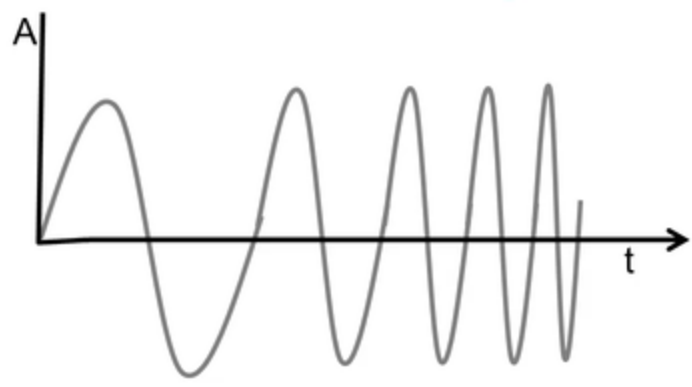
\includegraphics[ width=0.7\linewidth, keepaspectratio]{chirp_a_vs_t.png}
			\caption{Linearly modulated sinusoidal signal known as a chirp. Modulates from frequency $f_c$ to $f_c + B$ \cite{tiPresentation}.}
			\label{fig:chirp_a_vs_t}
		\end{figure} %

		\begin{figure}[tbp]
			\centering
			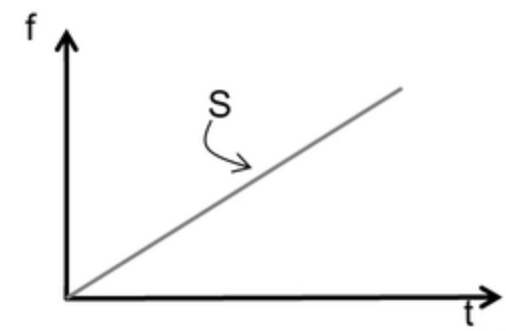
\includegraphics[ width=0.7\linewidth, keepaspectratio]{chirp_f_vs_t.png}
			\caption{Chirp in a frequency vs time plot showing the linear modulation with slope $S$ \cite{tiPresentation}.}
			\label{fig:chirp_f_vs_t}
		\end{figure} %

		FMCW radars generate a sinusoidal signal whose frequency is linearly modulated over bandwidth $B$ from the center frequency $f_c$ to $f_c + B$ as shown in \autoref{fig:chirp_a_vs_t}. This signal is known as a chirp. The rate of increase $S$ in the frequency, also known as sweep rate, is given in MHz/s. The time span over which the signal is modulated is given by $T_c$ in seconds. \autoref{fig:chirp_f_vs_t} shows the frequency of the chirp over time.

		\begin{figure}[tbp]
			\centering
			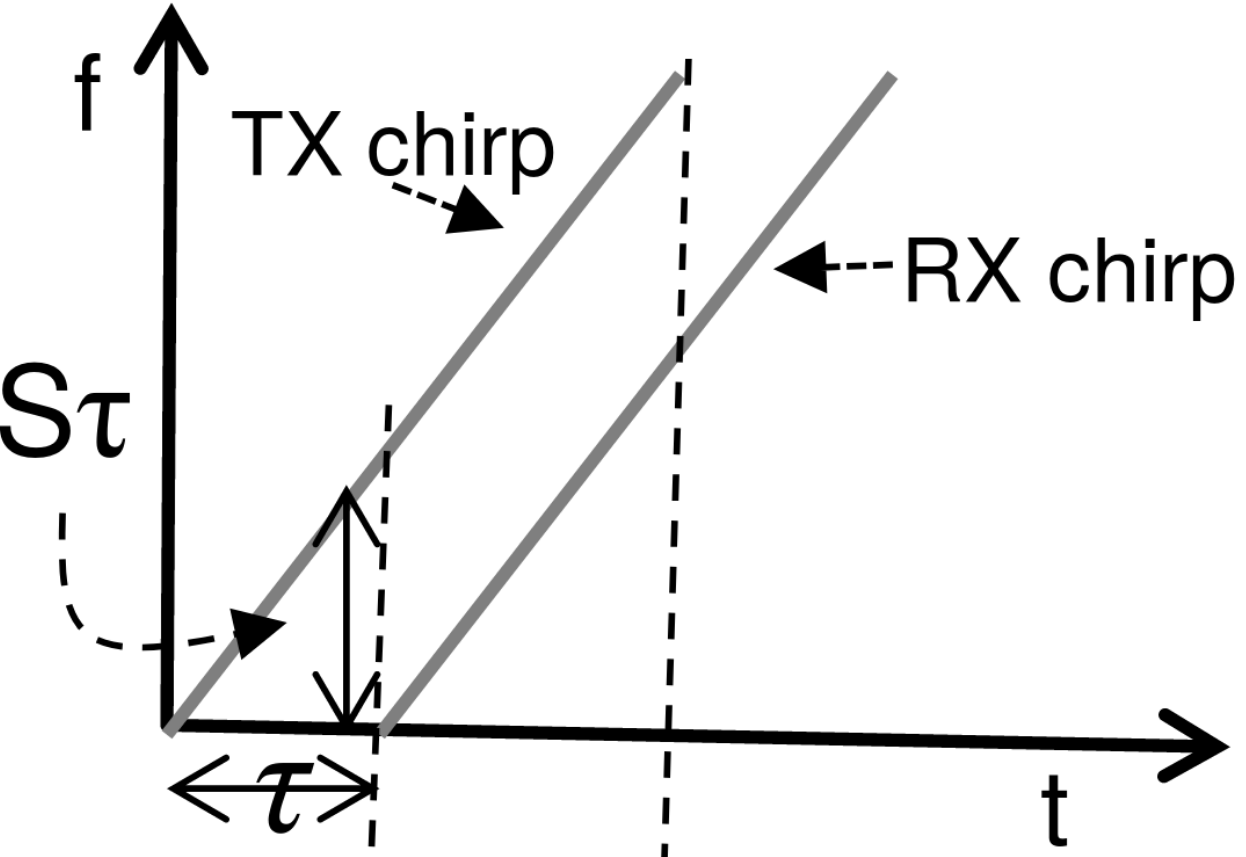
\includegraphics[ width=0.7\linewidth, keepaspectratio]{tx_rx_chirp.png}
			\caption{Showcasing time difference $\tau$ between transmitted and received chirp \cite{tiPresentation}.}
			\label{fig:tx_rx_chirp}
		\end{figure} %

		The receiver modules then receive the chirp after it has traveled to an object and bounced back. The time difference between when the chirp is first transmitted and when it is first received is given by $\tau$. The signal being transmitted at time $t$ has the frequency $\omega_1$ while the signal being received at the same time has frequency $\omega_2$. By sending the currently transmitted and received chirps through a mixer, an Intermediate Frequency (IF) signal is produced. The instantaneous frequency of the IF signal is the difference of the instantaneous frequencies of the two chirps. The frequency of the IF signal $S_{\tau}$ is then $\frac{S2d}{c}$. This value is a constant as the difference between the transmitted and received chirps will always be the same. The IF signal can be determined using the transmit chirp $x_{TX}$ and the receive chirp $x_{RX}$ to create $x_{IF}$ as follows:
		\begin{align}
			x_1 	&= \text{sin}[\omega_1t + \phi_1] \label{eq:x1} \\
			x_2 	&= \text{sin}[\omega_2t + \phi_2] \label{eq:x2} \\
			x_{out} &= \text{sin}[(\omega_1 - \omega_2)t + (\phi_1 - \phi_2)]. \label{eq:xout}
		\end{align}

		Using the frequency of the IF signal $f_{IF}$, the distance of an object $d$ can be calculated using the equation
		\begin{equation}
			d = \frac{cf_{IF}}{2S}.
		\end{equation}

		Since the received chirp will bounce off both the surface of the tread and the grooves from different angles, the resulting received chirp will have multiple frequency components. Each of these components will correspond to different points on the tire. It is important to differentiate these points to form an accurate mapping of the surface of the tire. 

			\begin{figure}[tbp]
				\centering
				\begin{subfigure}[b]{\linewidth}
					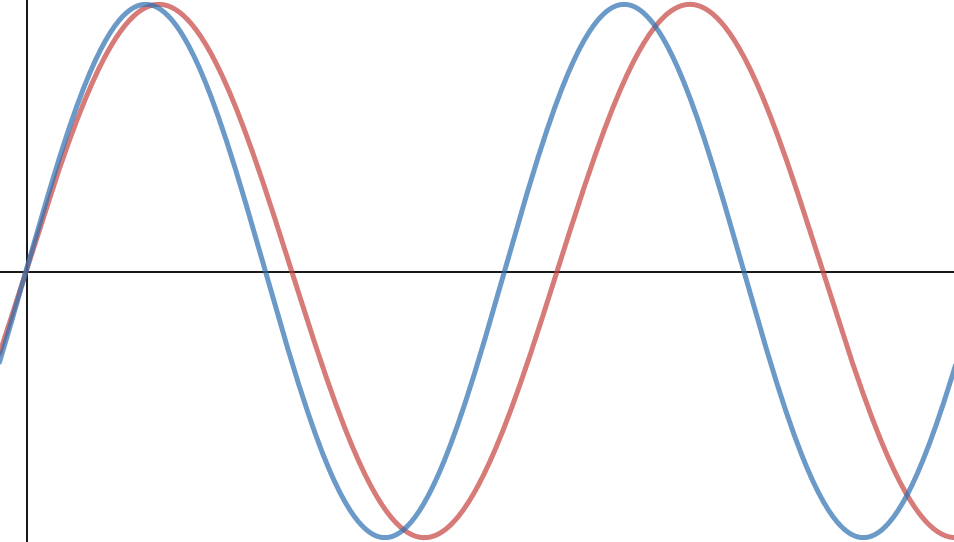
\includegraphics[width=0.5\linewidth,keepaspectratio]{shortSine.png}
					\caption{}
					\label{fig:shortSine}
				\end{subfigure} %
				\begin{subfigure}[b]{\linewidth}
					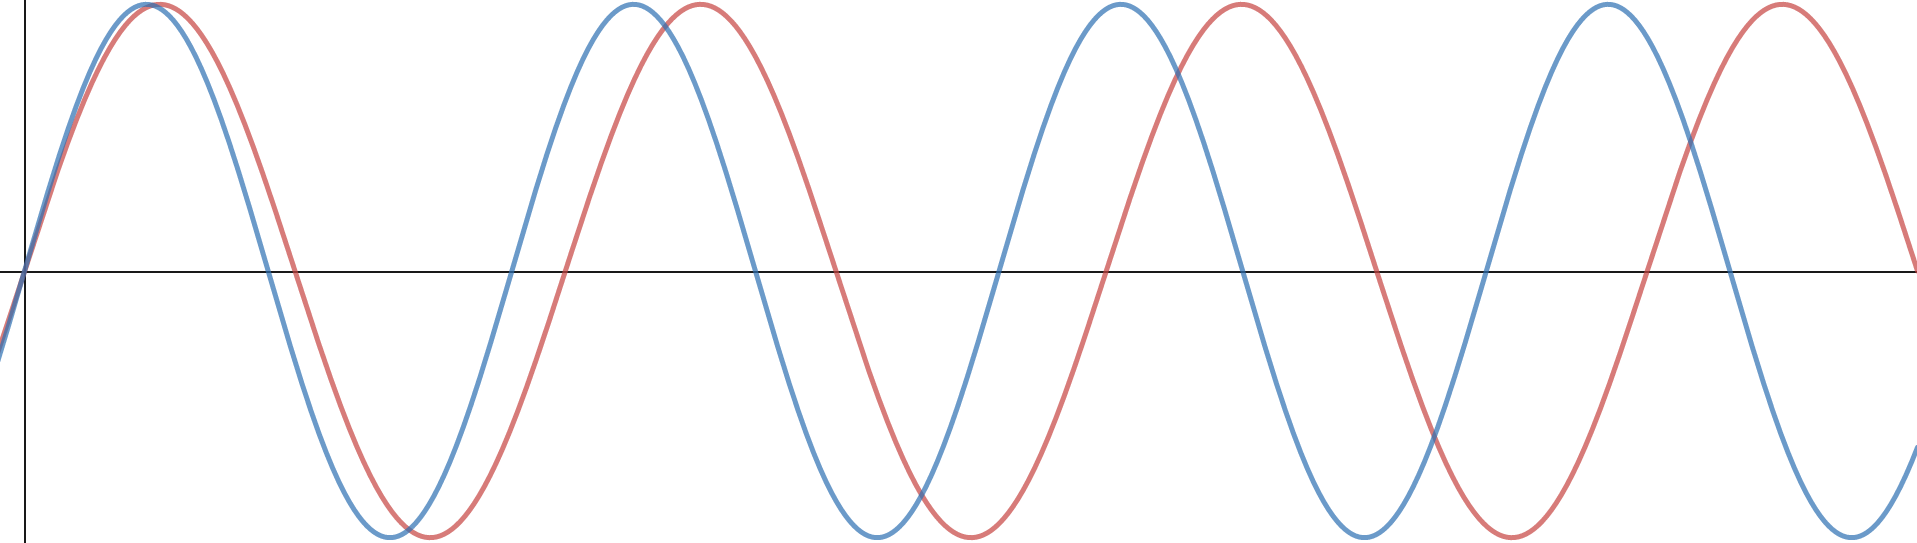
\includegraphics[width=\linewidth,keepaspectratio]{longSine.png}
					\caption{}
					\label{fig:longSine}
				\end{subfigure} %
				\caption{Observing a fewer number of cycles (a) versus observing more cycles (b) does not give enough resolution to determine the difference between two objects.}
				\label{fig:LongvShortSine}
			\end{figure}%

		By performing a fourier transform of the chirp, the different frequency components will be determined. However, because of the very small difference in distance between the surface of the tread and the grooves, these frequencies will be very close together. To be able to differentiate between these frequencies, a long observation window is required. By increasing the observation window time, the range resolution increases. This can be seen by comparing the plots of two sine waves with similar, but different frequencies over a short period of time, \autoref{fig:shortSine}, and over a longer period of time, \autoref{fig:longSine}. From these figures, it is obvious that a longer observation window shows the sine waves are significantly different, implying multiple objects at different distances.

		Using all of this information provides us with a distance to an object. However, this does not provide us with a direction to the object. That is, finding the frequencies of the received chirps will tell us how far away objects are, but not whether they are to the right or to the left of us. To do this, we need to estimate the Angle of Attack (AoA) of the received signals. This is done by comparing the signals received at at least two different receivers. This is the same concept as stereo vision where having two or more perspectives allows for depth perception by comparing the information the two receivers receive. 

		\begin{figure}[tbp]
			\centering
			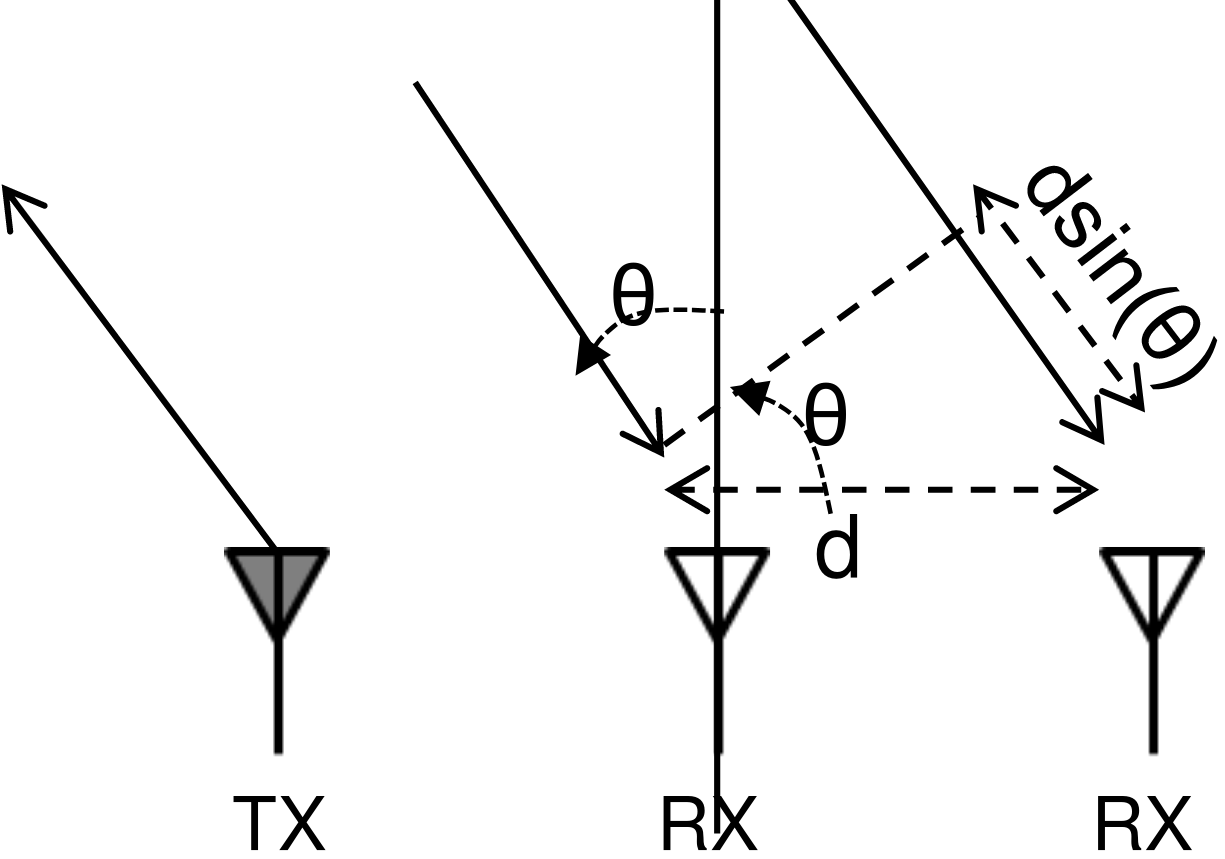
\includegraphics[ width=0.7\linewidth, keepaspectratio]{aoaFig.png}
			\caption{Angle of attack showcase using one transmitter and two receivers \cite{tiPresentation}.}
			\label{fig:aoa}
		\end{figure} %

		Each of the receivers perform a 2-dimensional FFT on the received data to produce a grid result where signals are binned based on range and velocity. For each receiver, signals in the same location will have frequency peaks at the same point. However, they will have different phases due to their incoming AoA for each receiver. The phase difference between these two signals is given by $\omega$. Then, the AoA, given by $\theta$, can be calculated using $\omega = \frac{2\pi\text{sin}(\theta)}{\lambda}$. This can be derived from \autoref{fig:aoa} which shows two receiver modules receiving a chirp bounced from the same object. 

		\begin{figure}[tbp]
			\centering
			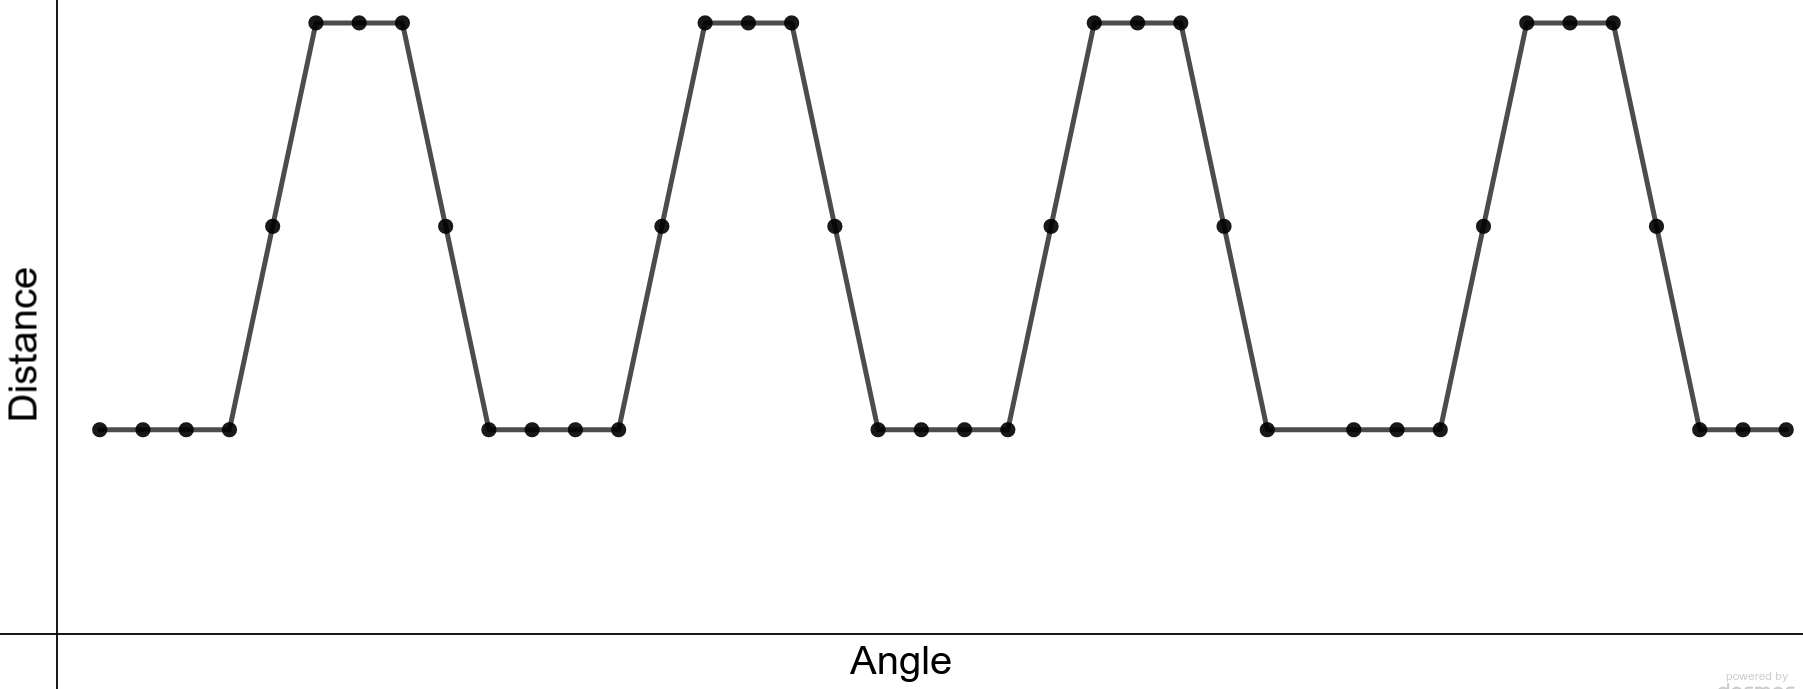
\includegraphics[ width=\linewidth, keepaspectratio]{treadMap.png}
			\caption{Example tread mapping where the y-axis is the distance from the sensor and the x-axis is the angle to the sensor. The peaks are the grooves in the tire (further away) while the points in the troughs represent the surface of the tread (close to the sensor).}
			\label{fig:treadMap}
		\end{figure} %

		Combining the AoA information with the range detection, data points can be collected horizontally across the tire as other data is filtered out. This data can be plotted to form a mapping of the surface of the tread on the tire. An example of this is shown in \autoref{fig:treadMap}. This plot shows the distance at points on the tread of the tire where points further away represent the grooves and points closer to the sensor represent the surface of the tread. The x-axis represents the angle of attack from the measured point to the sensor. 

		The system will then take an average of the high points and the low points and find the difference between the two. This gives an average tread depth reading. If this value is outside of the acceptable range (usually less than 3/32'' on passenger vehicles), then the user will be notified that the tread depth is dangerously low. This notification will likely take the form of an LED within the car itself. Further integration into the dashboard is possible, but requires significant customization of the vehicle until car manufacturers adopt tread awareness systems as standard.


	\section{Parts List}
		Since the design has not yet been finalized, the parts list is not complete. \autoref{tab:parts} shows the current expected parts required for the FMCW radar-based design. An FMCW radar sensor is required to collect the sensing data. The two most promising options are the AWR1642 \cite{AWR1642} and IWR1642 \cite{IWR1642} booster packs available from Texas Instruments. When a final decision has been made on the exact sensor, the table will be updated with specific information.

		A microcontroller is required to take the data from the FMCW sensor before performing calculations to determine distance measurements. These distance measurements are then plotted to determine the average tread depth of the tire. The microcontroller will then communicate with a simple LED to signal the driver that the tread depth is low (LED on) or that the tread depth is safe (LED off). For the Texas Instruments family of sensors, an MSP432 LaunchPad environment is able to communicate with the booster packs using Texas Instruments' mmWave software development kit.

		\begin{table}[t]
			\begin{center}
				\caption{Parts required for ATIS using a radar sensor.}
				\label{tab:parts}
				\begin{tabular}{l|l}
					Part 			& Quantity  \\
					\hline
					\vspace{-0.1in}		&	\\
					FMCW Radar Sensor 	& 1 \\
					Red LED 			& 1 \\
					Microcontroller		& 1 
				\end{tabular}
			\end{center}
		\end{table}


	\section{Prototype and System Integration}
		By the end of this semester, our expectation is to have a working prototype of an FMCW radar sensor to map the surface of a tire. The sensor will send the data to a microcontroller that will then determine the approximate tread depth. The controller will then send a notification signal (likely through an LED for prototyping) to alert a driver if the tread depth is outside of a specified range.

		Once these functionalities are implemented, the sensor will be improved to measure with a higher accuracy. Then, functional tests on a real vehicle will be conducted. From this point, optimization and further testing will be conducted to improve the device. The housing of the sensor will also be improved so that inclement weather, rough terrain, and dirt do not degrade the measurements taken. Through this process, the sensor will be made with off-the-shelf parts to stay within budget and produce a working final product.


	\section{Deliverables}
		Once the product itself is complete, we will compose a final report discussing our findings, results, and conclusions. This report will discuss the specifics of the final product, the difficulties in completing it, and the specific details of how it functions. A poster and presentation will also be prepared to give a high-level understanding of the product and how it functions to business leaders, professors, and peers.


	\section{Timeline}
		To ensure the timely completion of the project, three Gantt charts have been created. These charts supply us with expected milestones for the project. This allows us to visually determine whether or not we are on schedule to complete the project. The Gantt chart is a constantly adjusting figure that will become more specific as the design for the product is further refined. \autoref{fig:ganttChartSP2020}, \autoref{fig:ganttChartSU2020}, and \autoref{fig:ganttChartFA2020} are the Gantt charts outlining our planned tasks over the spring, summer, and fall of 2020, respectively.

		\begin{figure*}[t]
			\centering
			\begin{ganttchart}[y unit title=0.5cm, y unit chart=0.6cm, x unit=0.75cm, vgrid, hgrid, title label anchor/.style={below=-1.6ex}, title left shift=0, title right shift=0, title height=1, bar/.style={fill=gray!50}, incomplete/.style={fill=white}, progress label text={}, bar height=0.5, group right shift=0, group top shift=.6, group height=.3]{1}{17}
				% Month labels
				\gantttitle{January}{3}
				\gantttitle{February}{4} 
				\gantttitle{March}{5} 
				\gantttitle{April}{4} 
				\gantttitle{May}{1}  \\

				% First day of week labels
				\gantttitle{13}{1}
				\gantttitle{20}{1}
				\gantttitle{27}{1}

				\gantttitle{3}{1}
				\gantttitle{10}{1}
				\gantttitle{17}{1}
				\gantttitle{24}{1}

				\gantttitle{2}{1}
				\gantttitle{9}{1}
				\gantttitle{16}{1}
				\gantttitle{23}{1}
				\gantttitle{30}{1}

				\gantttitle{6}{1}
				\gantttitle{13}{1}
				\gantttitle{20}{1}
				\gantttitle{27}{1}

				\gantttitle{4}{1} \\

				% Tasks
				\ganttbar{Project Proposal}{1}{14} \\
				\ganttbar{Sensor Design}{2}{12} \\
				\ganttbar{Housing Design}{4}{7} \\
				\ganttbar{Alert System Design}{8}{12} \\
				\ganttbar{Order Parts}{13}{17} \\
				\ganttbar{Initial Construction}{14}{16} \\
				\ganttbar{Redesign}{15}{17}

				% Relations 
				% \ganttlink{elem1}{elem4}
				% \ganttlink{elem2}{elem4}
				% \ganttlink{elem3}{elem4}
			\end{ganttchart}
			\caption{Tasks for Spring 2020.}
			\label{fig:ganttChartSP2020}
		\end{figure*}

		\begin{figure*}[t]
			\centering
			\begin{ganttchart}[y unit title=0.5cm, y unit chart=0.6cm, x unit=0.85cm, vgrid, hgrid, title label anchor/.style={below=-1.6ex}, title left shift=0, title right shift=0, title height=1, bar/.style={fill=gray!50}, incomplete/.style={fill=white}, progress label text={}, bar height=0.5, group right shift=0, group top shift=.6, group height=.3]{1}{15}
				% Month labels
				\gantttitle{May}{3}
				\gantttitle{June}{5} 
				\gantttitle{July}{4} 
				\gantttitle{August}{3} \\

				% First day of week labels
				\gantttitle{11}{1}
				\gantttitle{18}{1}
				\gantttitle{25}{1}

				\gantttitle{1}{1}
				\gantttitle{8}{1}
				\gantttitle{15}{1}
				\gantttitle{22}{1}
				\gantttitle{29}{1}

				\gantttitle{6}{1}
				\gantttitle{13}{1}
				\gantttitle{20}{1}
				\gantttitle{27}{1}

				\gantttitle{3}{1}
				\gantttitle{10}{1}
				\gantttitle{17}{1} \\

				% Tasks
				\ganttbar{Redesign}{1}{3} \\
				\ganttbar{Testing}{3}{8} \\
				\ganttbar{\quad\quad\enspace Final Redesign}{8}{15}

				% Relations 
				% \ganttlink{elem0}{elem1}
			\end{ganttchart}
			\caption{Tasks for Summer 2020.}
			\label{fig:ganttChartSU2020}
		\end{figure*}

		\begin{figure*}[t]
			\centering
			\begin{ganttchart}[y unit title=0.5cm, y unit chart=0.6cm, x unit=0.796875cm, vgrid, hgrid, title label anchor/.style={below=-1.6ex}, title left shift=0, title right shift=0, title height=1, bar/.style={fill=gray!50}, incomplete/.style={fill=white}, progress label text={}, bar height=0.5, group right shift=0, group top shift=.6, group height=.3]{1}{16}
				% Month labels
				\gantttitle{August}{2}
				\gantttitle{September}{4} 
				\gantttitle{October}{4} 
				\gantttitle{November}{5} 
				\gantttitle{Dec.}{1}  \\

				% First day of week labels
				\gantttitle{24}{1}
				\gantttitle{31}{1}

				\gantttitle{7}{1}
				\gantttitle{14}{1}
				\gantttitle{21}{1}
				\gantttitle{28}{1}

				\gantttitle{5}{1}
				\gantttitle{12}{1}
				\gantttitle{19}{1}
				\gantttitle{26}{1}

				\gantttitle{2}{1}
				\gantttitle{9}{1}
				\gantttitle{16}{1}
				\gantttitle{23}{1}
				\gantttitle{30}{1}

				\gantttitle{7}{1} \\

				% Tasks
				\ganttbar{Final Redesign}{1}{2} \\
				\ganttbar{Product Testing}{1}{14} \\
				\ganttbar{Implementation}{3}{14} \\
				\ganttbar{Optimization}{4}{12} \\
				\ganttbar{\quad Final Presentation}{12}{16}

				% Relations 
				% \ganttlink{elem0}{elem1}
			\end{ganttchart}
			\caption{Tasks for Fall 2020.}
			\label{fig:ganttChartFA2020}
		\end{figure*}

		\subsection{Teamwork}
			The timeline of the project can be broken into various phases. Although each team member will provide an equal amount of contribution, each will take a lead on a different phase of the project. The key project phases along with leaders of each phase is shown in \autoref{tab:phaseLeaders}. The ultimate goal is to be completed with the design of our prototype after the first semester. This will allow for testing and further optimization of the product during the implementation phase. This timeline will also allow extra time for unexpected issues that will arise during implementation.

			\begin{table}[tb]
				\centering
				\begin{tabularx}{\linewidth}{l|l}
					Project Phase 						& Leader \\
					\hline
					\vspace{-0.1in}						& \\
					Research 							& Nicholas Chiapputo \\
					Project Definition					& Brandon Jones \\
					Specification and Requirements 		& Tim McCoig \\
					Design and Algorithm Development 	& Nicholas Chiapputo \\
					Testing and Optimization 			& Brandon Jones \\
					Prototype Implementation 			& Samuel Simmons
				\end{tabularx}
				\caption{Leaders for each key project phase.}
				\label{tab:phaseLeaders}
			\end{table}


	\begin{thebibliography}{00}
		% Statistics on car crashes
		\bibitem{cdcKeyStats} Center for Disease Control and Prevention, ``Key Data and Statistics,'' 2015. [Online]. Available: \url{https://www.cdc.gov/injury/wisqars/overview/key_data.html}

		\bibitem{nhtsaCrashStats} National Highway Traffic Safety Administration, ``Tire-Related Factors in the Pre-Crash Phase,'' 2012. [Online]. Available: \url{https://crashstats.nhtsa.dot.gov/Api/Public/ViewPublication/811617}


		% Patents for tread sensing
		% \bibitem{justwheelsPatent} T. Scheckter, ``Radar tread sensing for wheel well,'' U.S. Patent 20200031173A1, Jul., 19, 2019. 
		
		\bibitem{continentalPatent} T. A. Brey, ``Tire tread wear sensor system,'' U.S. Patent 7180409B2, Feb., 20, 2007.
		
		\bibitem{intellitread} ``Tire Tread Wear Sensors - Tyrata.'' Accessed on: Feb. 11, 2020. [Online]. Available: \url{https://tyrata.com/}
		
		\bibitem{goodyearPatent1} C. T. R. Pulford, C. H. Lin, ``Sensor system for monitoring tire wear,'' U.S. Patent 20190184763A1, Dec., 19, 2018.
		
		\bibitem{nxpbvPatent} R. L. Robinson, ``System and method for determining tread wear of a tire,'' U.S. Patent 9831922B1, Nov., 28, 2017.
		
		\bibitem{goodyearPatent2} M. Engel, B. W. Kimble, and D. Lednik, ``Tire tread wear sensor system,'' U.S. Patent 20160075189A1, Mar., 17, 2014.
		
		\bibitem{patent4} R, Achterholt, ``Method and device for detecting the wear on at least one tire of a vehicle,'' U.S Patent 20190344625A1, Nov., 14, 2019.

		% SiGe papers
		\bibitem{122ghz} S. Scherr, \textit{et al.}, ``Miniaturized 122 ghz ism band fmcw radar with micrometer accuracy,'' In \textit{2015 European Radar Conference (EuRAD)}, Paris, 2015, pp. 277-280.

		\bibitem{240ghz} T. Jaeschke, C. Bredendiek, N. Pohl. ``A 240 ghz ultra-wideband fmcw radar system with on-chip antennas for high resolution radar imaging,'' In \textit{2013 IEEE MTT-S International Microwave Symposium Digest (MTT)}, Seattle, WA, 2013, pp. 1-4.
    	

		% Standards
    	\bibitem{80215standard} \textit{Standard for Low-Rate Wireless Networks - Amendment 5: Enabling/Updating the Use of Regional Sub-GHz Bands}, IEEE Standard 802.15.14v-2017, IEEE Computer Society, New York, 2017.
		
		\bibitem{1451standard} \textit{Standard for a Smart Transducer Interface for Sensors and Actuators - Wireless Communication and Transducer Electronic Data Sheet (TEDS) Formats}, IEEE Standard 1451.5-2007, IEEE Instrumentation and Measurement Society, New York, 2007. 


		% Products
		\bibitem{A111} ``SparkFun Pulsed Radar Breakout - A111.'' SparkFun. \url{https://www.sparkfun.com/products/15577} (accessed Mar. 9, 2020).

		
		% TI presentation on FMCW 
		\bibitem{tiPresentation} S. Rao. Introduction to mmwaveSensing: FMCW Radars [PDF]. Available: \url{https://training.ti.com/sites/default/files/docs/mmwaveSensing-FMCW-offlineviewing_2.pdf}.


		% Potential FMCW sensor boards
		\bibitem{AWR1642} AWR1642BOOST mmWave Sensor. Texas Instruments. \url{https://www.ti.com/tool/AWR1642BOOST} (accessed Mar. 9, 2020).

		\bibitem{IWR1642} IWR1642BOOST mmWave Sensor. Texas Instruments. \url{https://www.ti.com/tool/IWR1642BOOST} (accessed Mar. 9, 2020).
		
		\bibitem{roleOfmmWave} A. Bhutani, S. Marahrens, M. Gehringer, B. G{\"o}ttel, M. Pauli, T. Zwick, ``The role of millimeter-waves in the distance measurement accuracy of an fmcw radar sensor,'' \textit{Sensors 2019}, vol. 19, no. 18, Sept., 2019, doi: 10.3390/s19183938.
	\end{thebibliography}
\end{document}